\documentclass[11pt]{article}
\usepackage[utf8]{inputenc}
\usepackage[T1]{fontenc}
\usepackage{lmodern}
\usepackage{amsmath,amssymb}
\usepackage{float}
\usepackage[a4paper, margin=2.0cm, headheight=13pt]{geometry}
\usepackage{graphicx}
\graphicspath{{../../evaluation/results/2026-11-16/figures/}}
\usepackage{booktabs}
\usepackage{array}
\usepackage{tabularx}
\usepackage{enumitem}
\usepackage{xcolor}
\usepackage{tikz}
\usetikzlibrary{positioning,arrows.meta,fit,backgrounds}
\usepackage{caption}
\usepackage{fancyhdr}
\usepackage{hyperref}
\hypersetup{colorlinks=true, linkcolor=black, urlcolor=blue!50!black, citecolor=black,
  pdftitle={Secure Multi-Tenant Identity and Access Platform: Project Report}, pdfauthor={Team P01-G33}}
\setlist{itemsep=1pt, topsep=3pt, leftmargin=1.3em}
\renewcommand{\arraystretch}{1.18}
\setlength{\parskip}{3pt}
\setlength{\parindent}{0pt}
\setlength{\emergencystretch}{3em}
\newcolumntype{L}{>{\raggedright\arraybackslash}X}
\newcolumntype{P}[1]{>{\raggedright\arraybackslash}p{#1}}
\captionsetup{font=small, labelfont=bf, skip=4pt}
\pagestyle{fancy}
\fancyhf{}
\fancyhead[L]{\small Secure Multi-Tenant IAM Platform --- Project Report}
\fancyhead[R]{\small Team P01-G33 \textperiodcentered{} CS5903}
\fancyfoot[C]{\small\thepage}
% Non-code contributions of Jaya Prakash, as stated by the team (empty until confirmed).
\newcommand{\JayaContribution}{}
\newcommand{\code}[1]{\texttt{\small #1}}
\newcommand{\repo}{https://github.com/krishnateja2314/iam-provider}
\newcommand{\gh}[2]{\href{\repo/blob/cs5903-final-2026/#1}{#2}}
\newcommand{\commit}[1]{\href{\repo/commit/#1}{\texttt{#1}}}

\makeatletter
\renewcommand\section{\@startsection{section}{1}{0pt}{-10pt plus -2pt}{4pt}{\large\bfseries}}
\renewcommand\subsection{\@startsection{subsection}{2}{0pt}{-7pt plus -2pt}{2pt}{\normalsize\bfseries}}
\makeatother
\begin{document}

%% ---------------------------------------------------------------- Cover
\begin{center}
{\small Indian Institute of Technology Hyderabad \textperiodcentered{} CS5903 Distributed AI Training (DAT) \textperiodcentered{} Final Project Report}\\[6pt]
{\LARGE\bfseries Secure Multi-Tenant Identity and Access Platform}\\[4pt]
{\large for a learning SaaS, with user-delegated AI agents}\\[8pt]
\end{center}
\begin{tabularx}{\textwidth}{@{}P{3.6cm} L@{}}
\toprule
Project ID / group no. & Project 01 \textperiodcentered{} Group 33 (team P01-G33)\\
Members & Krishna Teja (CS23BTECH11028) \textperiodcentered{} Jaya Prakash (CS23BTECH11015)\\
Mentor / instructor & Koundinya \textperiodcentered{} Prof.\ Praveen Tammana\\
Repository & \url{\repo}\\
Final tag / code revision & \texttt{cs5903-final-2026} \textperiodcentered{} verified code revision \commit{e13f019} (the tag adds only documentation, evaluation scripts and results; \code{backend/}, \code{clients/} and \code{infrastructure/} are byte-identical)\\
Demo & recorded walkthrough \gh{docs/demo/demo-walkthrough.mp4}{\code{docs/demo/demo-walkthrough.mp4}}; no public deployment (local Docker lab)\\
Date & 16 November 2026\\
\bottomrule
\end{tabularx}

\subsection*{Executive summary}
\textbf{Problem.} In a multi-tenant learning SaaS one person can be an \emph{admin} in one organization and a \emph{learner} in another, and programs (AI agents) increasingly act for users. Common shortcuts leak access: trusting a client-sent tenant ID, roles cached in tokens, email-based account merging, ``valid until expiry'' tokens, and audit that can silently fail.
\textbf{Delivered.} A working modular-monolith platform (Node.js 24, Fastify 5, PostgreSQL 16) in which Keycloak 26.8.0 proves \emph{who} a person or program is (OIDC + S256 PKCE, enterprise brokering) and our backend decides, per tenant and per request, \emph{what} it may do. That covers memberships, Casbin deny-overrides, relationship rules, provisioning, consent, transactional audit, an application service principal (AG01) and a user-delegated agent (AG02) whose permission is \emph{user} $\cap$ \emph{scope} $\cap$ \emph{tenant}.
\textbf{What works today.} From a clean clone, 253/253 tests pass with a live provider. 15/15 deliberately injected security bugs are caught. A real-browser proof passes 11/11 on two host names. Against the JWT-only baseline, which accepted a revoked token in 15/15 trials (59.4\,s median for agent tokens), our API refused it on the first request in 15/15 trials.
\textbf{Completion.} All seven milestones M1--M7 and both agent extensions are \emph{implemented and verified}. M5 is the agreed minimal slice, not full SCIM. Not done: an independent second-machine rerun, native mobile apps, production hardening (\S8).

%% ---------------------------------------------------------------- 1
\section*{1. Problem, scope \& success criteria}
\textbf{Actors.} Learners, instructors and tenant admins (several tenants per person); a platform admin (provisioning only); enterprise users signing in through their company IdP; an AG01 reporting agent (acts as itself); an AG02 assistant agent (acts for one user). Adversaries (Week 1 threat model): an unauthenticated attacker, a member of another tenant, a compromised or revoked user, a holder of a stolen token, an over-privileged agent, and a client sending malformed claims.

\textbf{Problem statement.} Separate authentication, profile, tenant membership and authorization, and \emph{prove with tests that can fail} that tenant and privilege boundaries hold for both humans and agents.

\textbf{In scope:} OIDC sign-in on web and a mobile-style client, an enterprise broker, the session lifecycle, fine-grained authorization, minimal provisioning, consent and audit, and both agents. \textbf{Out of scope:} our own OIDC server, native apps, full SCIM~2.0, real corporate IdPs/SAML, production deployment. \textbf{Assumptions/constraints:} the IdP, database and backend host are trusted; local HTTP lab with synthetic data and public development credentials; eight weeks, two students.

\begin{table}[H]
\centering\small
\begin{tabularx}{\textwidth}{@{}l P{3.3cm} L@{}}
\toprule
\textbf{ID} & \textbf{Milestone} & \textbf{``Done when'' (frozen acceptance test / target metric)}\\
\midrule
M1 & Identity \& tenant model & users, identities, profiles, orgs, memberships, roles are separate; 12 concurrent first logins $\Rightarrow$ 1 user; no email merge\\
M2 & Sign-in \& federation & PKCE login on web + mobile client and enterprise broker in a real browser (11/11 checks, 2 hosts)\\
M3 & Session lifecycle & logout/revocation $\Rightarrow$ 401 on the \emph{first} request ($\le$5\,s); refresh replay kills the family; reset alone does not revoke\\
M4 & Fine-grained authorization & declarative policy over $\ge$40 scenarios (59 delivered); RBAC + ABAC + ReBAC; deny-overrides\\
M5 & Tenant provisioning & idempotent create, admin bootstrap, quotas, suspend/reactivate, tenant SSO domain, one transaction\\
M6 & Consent \& audit & purpose-specific append-only consent; field allowlist; audit rolls back with the change\\
M7 & Security validation & cross-tenant, escalation, revoked-session, malformed-claim tests; every guard mutation killed\\
AG01 / AG02 & Agent extensions & one exact grant in one tenant / effective permission = user $\cap$ scope $\cap$ tenant; revocation on next request\\
\bottomrule
\end{tabularx}
\caption{Approved milestones and their frozen acceptance criteria (\gh{docs/evaluation-protocol.md}{\code{docs/evaluation-protocol.md}}, frozen 10 Oct 2026).}
\end{table}
\textbf{End-to-end ``done when'' workflow:} \code{docker compose up -d --build --wait} on a clean clone $\rightarrow$ Alice signs in with PKCE $\rightarrow$ admin in Acme (members 200), learner in Globex (members 403) $\rightarrow$ she delegates two scopes to the assistant agent, which gets 200 in scope, 403 on members and in the other tenant, and 401 after she revokes $\rightarrow$ sign-out makes her old token 401. This workflow is the recorded demo.

%% ---------------------------------------------------------------- 2
\section*{2. Related work, baselines \& alternatives}
Identity providers (Okta, Entra ID, Auth0, Keycloak, Ory, Zitadel, Authentik) implement OIDC/OAuth~2.0 well but leave tenant-aware, resource-specific decisions to the application. We follow OIDC Core~\cite{oidc} and the OAuth~2.0 Security BCP (RFC~9700: PKCE S256, refresh rotation, audience-restricted tokens)~\cite{bcp}. Relationship rules such as ``instructor teaches course'' are read at decision time, as in Zanzibar~\cite{zanzibar}. Provisioning follows the idempotent spirit of SCIM~\cite{scim}, consent and minimization the NIST Privacy Framework~\cite{nist}. For agents, token exchange (RFC~8693)~\cite{rfc8693} is the standard delegation format, and no settled practice exists for bounding an agent by its user's current rights.

\begin{table}[H]
\centering\small
\begin{tabularx}{\textwidth}{@{}P{3.2cm} P{4.6cm} L@{}}
\toprule
\textbf{Decision} & \textbf{Alternatives considered} & \textbf{Selected and why (ADR)}\\
\midrule
Architecture & 8 microservices (Week 0); plain monolith & modular monolith: one ACID transaction for change + audit, low 8-week risk (ADR-001)\\
Authentication & own OIDC server; Authentik/Ory; hosted IdP & Keycloak 26.8.0: standards, broker, realm-as-JSON, offline reproducible (ADR-002)\\
Authorization & Keycloak Authz Services; hand-written checks; OPA/SpiceDB & Casbin 5.51.1 over facts in our DB; tenant/relationship rules as hard boundaries (ADR-003)\\
Token checking & JWT-only; JWT + cached introspection & JWT + \emph{uncached} introspection, fail closed (ADR-005)\\
Agent delegation & RFC 8693 token exchange; copying user roles & delegation record re-read per decision, evaluated as the user (ADR-014)\\
\bottomrule
\end{tabularx}
\caption{Viable approaches and the selection. Full records: \gh{docs/Architecture_Decision_Records.md}{\code{docs/Architecture\_Decision\_Records.md}}.}
\end{table}

\textbf{Reused frameworks (versions, licences).} Keycloak 26.8.0 (Apache-2.0), PostgreSQL 16.15 (PostgreSQL licence), Node.js 24.21 (MIT), Fastify 5.12.8, Casbin 5.51.1 (Apache-2.0), jose 6.2.12, Kysely 0.29.6, pg 8.23.1 (all MIT), Vitest 5.0.3 and Playwright 1.63.0 (MIT / Apache-2.0). \textbf{What we added:} the whole application-side layer: identity mapping, the tenant context gate, hard boundaries, the policy adapter with deny-overrides, provisioning, consent, audit, the AG01/AG02 principal model, the realm configuration and its non-destructive updater, browser clients, 253 tests, a mutation runner and the evaluation scripts.

\textbf{Working baseline.} \textbf{B0 = JWT-only validation}: accept any access token whose RS256 signature, issuer, audience, expiry and \code{typ} verify. This is the shortcut many APIs ship, and it is exactly the first half of our own validator. For test quality, the \emph{revision baseline} is the Week~3 head \texttt{953a0aa} (160 passed, 1 failed, 6 skipped, no working mutation check). Each mutation M1--M15 is a guard-removed baseline.

%% ---------------------------------------------------------------- 3
\section*{3. Architecture \& implementation}
\begin{figure}[H]
\centering
\resizebox{\textwidth}{!}{%
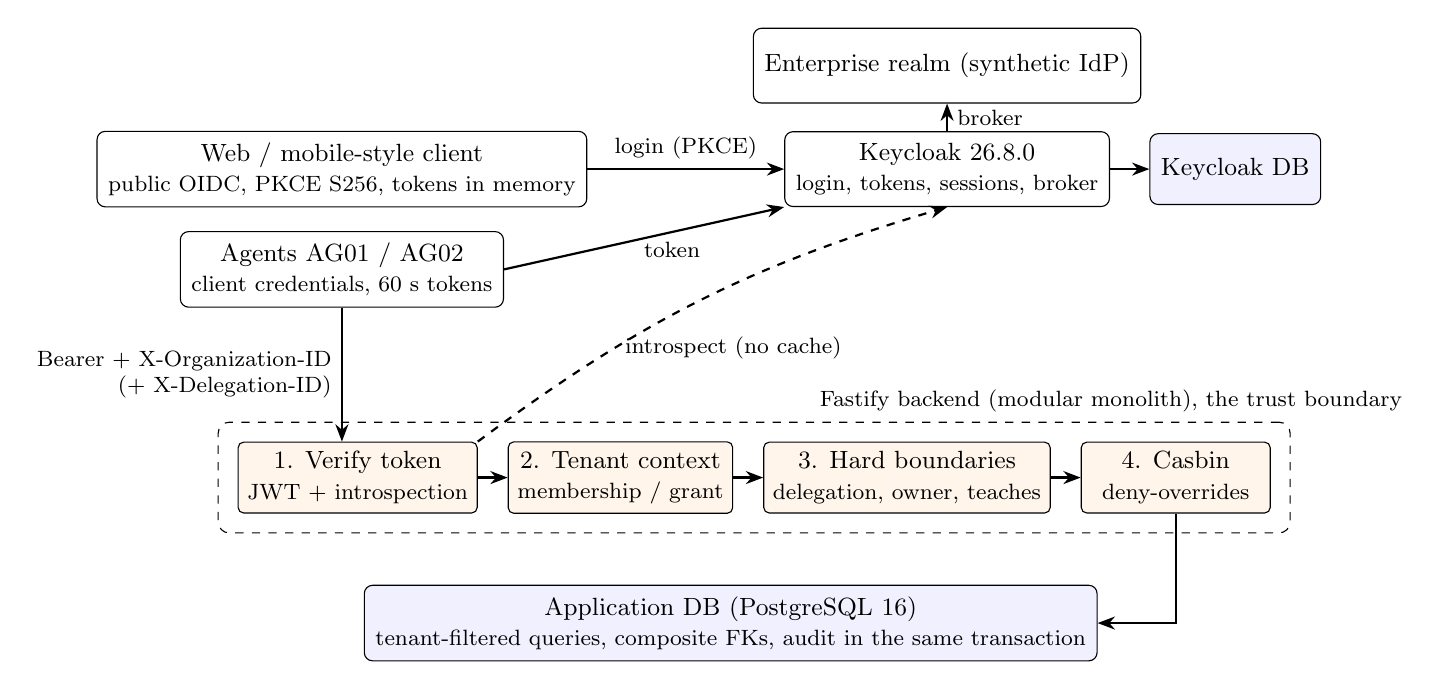
\begin{tikzpicture}[font=\small,
  box/.style={draw, rounded corners=3pt, align=center, minimum height=0.95cm, inner sep=4pt, fill=white},
  stage/.style={draw, rounded corners=2pt, align=center, minimum width=2.4cm, minimum height=0.9cm, fill=orange!8},
  db/.style={draw, rounded corners=3pt, align=center, minimum height=0.9cm, inner sep=4pt, fill=blue!6},
  arr/.style={-{Stealth[length=2.2mm]}, thick}, node distance=0.5cm and 0.38cm]
\node[box] (client) {Web / mobile-style client\\\footnotesize public OIDC, PKCE S256, tokens in memory};
\node[box, below=0.3cm of client] (agent) {Agents AG01 / AG02\\\footnotesize client credentials, 60 s tokens};
\node[box, right=2.5cm of client] (kc) {Keycloak 26.8.0\\\footnotesize login, tokens, sessions, broker};
\node[db, right=0.5cm of kc] (kcdb) {Keycloak DB};
\node[box, above=0.35cm of kc] (ent) {Enterprise realm (synthetic IdP)};
\node[stage, below=1.7cm of agent, xshift=0.2cm] (s1) {1. Verify token\\\footnotesize JWT + introspection};
\node[stage, right=of s1] (s2) {2. Tenant context\\\footnotesize membership / grant};
\node[stage, right=of s2] (s3) {3. Hard boundaries\\\footnotesize delegation, owner, teaches};
\node[stage, right=of s3] (s4) {4. Casbin\\\footnotesize deny-overrides};
\begin{scope}[on background layer]
\node[draw, dashed, rounded corners=4pt, fit=(s1)(s4), inner sep=7pt, label={[font=\footnotesize]above right:Fastify backend (modular monolith), the trust boundary}] (api) {};
\end{scope}
\node[db, below=0.9cm of s2, xshift=1.4cm] (appdb) {Application DB (PostgreSQL 16)\\\footnotesize tenant-filtered queries, composite FKs, audit in the same transaction};
\draw[arr] (client) -- node[above, font=\footnotesize]{login (PKCE)} (kc);
\draw[arr] (kc) -- (kcdb);
\draw[arr] (kc) -- node[right, font=\footnotesize]{broker} (ent);
\draw[arr] (agent.east) -- node[below, font=\footnotesize, pos=0.6]{token} (kc.south west);
\draw[arr] (agent.south) -- node[left, font=\footnotesize, align=right]{Bearer + X-Organization-ID\\(+ X-Delegation-ID)} (s1.north -| agent.south);
\draw[arr] (s1) -- (s2); \draw[arr] (s2) -- (s3); \draw[arr] (s3) -- (s4);
\draw[arr, dashed] (s1.north east) to[bend left=10] node[right, font=\footnotesize, pos=0.3]{introspect (no cache)} (kc.south);
\draw[arr] (s4.south) |- (appdb.east);
\end{tikzpicture}}
\caption{Components and the protected request path. Five containers in Docker Compose; neither database exports a host port. Everything the client sends is untrusted. A failing stage stops the request with 400/401/403/404/503.}
\label{fig:arch}
\end{figure}

\begin{table}[H]
\centering\small
\begin{tabularx}{\textwidth}{@{}P{3.0cm} L P{3.9cm}@{}}
\toprule
\textbf{Component} & \textbf{Responsibility / interface} & \textbf{Source}\\
\midrule
Token validator & RS256, issuer, audience, expiry, \code{typ=Bearer}, claim shape; uncached introspection; 401 invalid, 503 provider down; service vs human principal & \gh{backend/src/modules/auth}{\code{modules/auth}}\\
Tenant gate & \code{X-Organization-ID} is untrusted; requires active membership in an active org (humans), a grant (AG01) or a matching delegation (AG02) & \gh{backend/src/middleware.ts}{\code{middleware.ts}}\\
Authorization engine & \code{authorize(subject, org, resource, action, id)}: hard boundaries, then Casbin over baseline + tenant \code{policy\_rules}; deny on error & \gh{backend/src/modules/authorization}{\code{modules/authorization}}\\
Domain modules & users/profiles/consent, organizations/memberships, learning resources and submissions, provisioning + SSO discovery, audit & \gh{backend/src/modules}{\code{modules/*}}\\
Agents & AG01 registry + exact grants; AG02 delegations (create/list/revoke; scopes from a fixed delegable list) & \code{service-principal}, \code{delegation}\\
Data store & 18 tables, 5 migrations; unique \code{(issuer, subject)}; cross-tenant triggers; append-only consent; delegation FK to membership & \gh{backend/src/db/migrations}{\code{db/migrations}}\\
Provider config & two realm imports; non-destructive updater; clients \code{iam-web}, \code{iam-mobile}, \code{iam-backend}, agents & \gh{infrastructure/keycloak}{\code{infrastructure/keycloak}}\\
\bottomrule
\end{tabularx}
\caption{Major components. The REST API has 25 routes under \code{/api/v1} plus \code{/health} and \code{/ready} ( \code{me}, \code{sessions}, \code{resources}, \code{submissions}, \code{members}, \code{policies}, \code{consents}, \code{audit-events}, \code{organizations}, \code{sso/discover}, \code{delegations}, \dots).}
\end{table}
\textbf{External dependencies and trust:} Keycloak (in the Compose stack) is the only external service; no paid APIs or keys. The identity provider, database and backend host are trusted; headers, IDs, bodies and unverified claims are not.

%% ---------------------------------------------------------------- 4
\section*{4. Methodology \& experiment setup}
\textbf{Evaluation questions.} Q1 do the frozen acceptance tests pass from a clean clone? Q2 can the tests fail (mutation)? Q3 is a revoked session/agent refused on the next request, compared with B0? Q4 what does the per-request check cost? Q5 does the real-browser flow hold on two host names? Q6 does AG02 never exceed its user?

\textbf{Workload and provenance.} Synthetic and committed in the repository: two realm imports and a seed with 3 tenants, 5 users, courses and submissions. Experiment E1 creates a fresh \code{eval-<uuid>} user per trial and deletes it afterwards. No external datasets, no personal data.

\textbf{Hardware and software.} One laptop with Windows~11, Docker Desktop (Linux containers); images \code{node:24.21.0-alpine}, \code{postgres:16.15-alpine}, \code{keycloak:26.8.0}; dependencies pinned by \code{package-lock.json}; Microsoft Edge through Playwright 1.63. There are no random seeds to fix: fixtures use fixed UUIDs.

\textbf{Experiment E1 (baseline vs solution).} Four operations: provider logout, admin logout-all, AG01 client disabled, and password reset as a \emph{control}. Each is repeated 5 times. After the operation, the same token is presented to B0 and to our API once immediately and then every 1\,s until it expires. Metrics: first-request outcome; time to 401; number of requests accepted afterwards; seconds of exposure. Thresholds (frozen protocol, criterion 3): 401 on the first request, $\le$\,5000\,ms, 0 accepted afterwards.

\textbf{Other runs.} The full suite and the mutation runner come from a fresh \code{git clone} of \texttt{e13f019} with new volumes (14 Nov). Latency: 3 runs $\times$ 200 sequential requests per series after 20 warm-up requests, inside the container. Commands: \gh{evaluation/README.md}{\code{evaluation/README.md}}; the one-shot clean run is \gh{evaluation/run-clean-evaluation.ps1}{\code{evaluation/run-clean-evaluation.ps1}}.

%% ---------------------------------------------------------------- 5
\section*{5. Results, observations \& analysis}
\subsection*{Q3: baseline vs solution (E1, 16 Nov 2026, 20 trials)}
\begin{table}[H]
\centering\small
\resizebox{\textwidth}{!}{\begin{tabular}{@{}lccccc@{}}
\toprule
\textbf{Operation (5 trials)} & \textbf{B0 1st req.} & \textbf{Ours 1st req.} & \textbf{Ours: time to 401} & \textbf{B0 accepted after} & \textbf{Ours accepted after}\\
\midrule
Provider logout & accepted 5/5 & \textbf{401} 5/5 & 22 ms (median) & 15/30 polls & \textbf{0}\\
Admin logout-all & accepted 5/5 & \textbf{401} 5/5 & 13 ms & 15/30 & \textbf{0}\\
AG01 client disabled & accepted 5/5 & \textbf{401} 5/5 & 7 ms & 298/313 (59.4 s) & \textbf{0}\\
Password reset (control) & accepted 5/5 & accepted 5/5 & --- & 15/30 & 15/30\\
\bottomrule
\end{tabular}}
\caption{E1 results. Raw: \gh{evaluation/results/2026-11-16/e1-baseline-revocation.jsonl}{\code{e1-baseline-revocation.jsonl}}, \gh{evaluation/results/2026-11-16/summary.csv}{\code{summary.csv}}. Human trials use the opt-in \code{iam-test} client, whose sessions end after 3\,s, so their polling stops early.}
\label{tab:e1}
\end{table}
\begin{figure}[H]
\centering
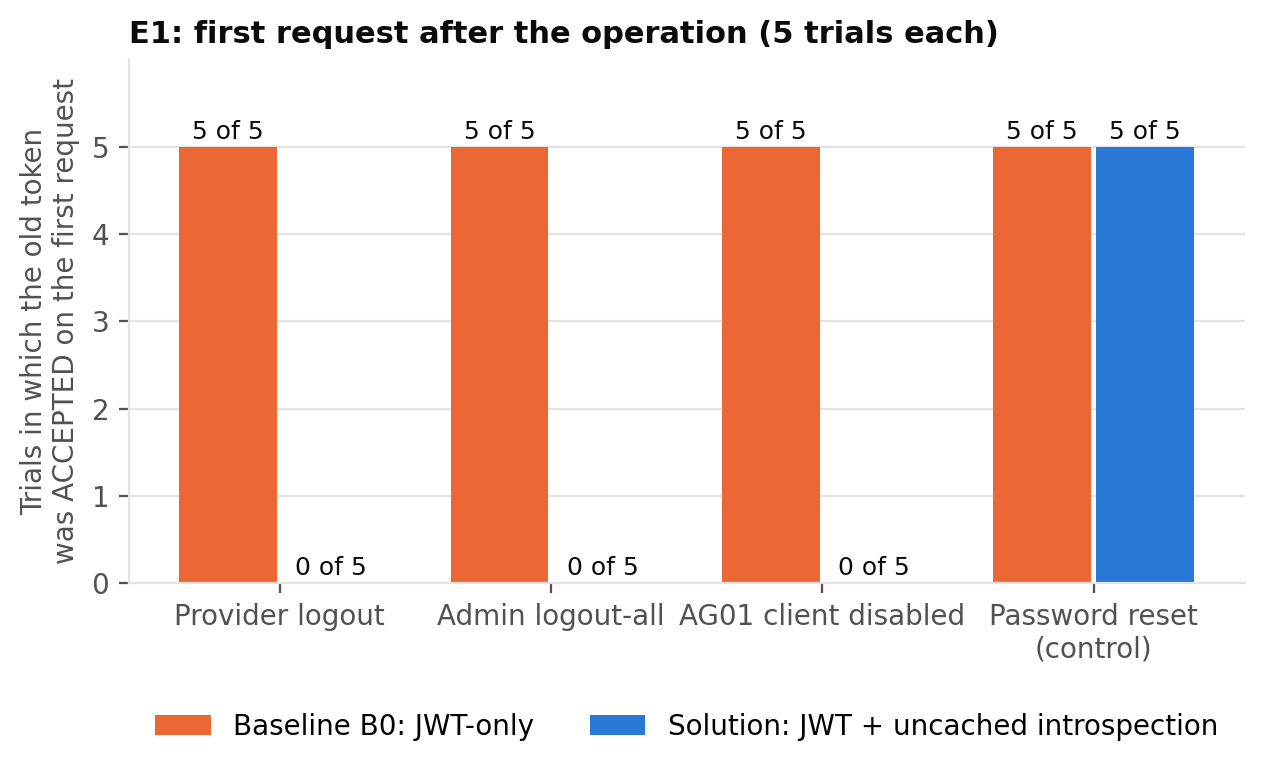
\includegraphics[width=0.49\textwidth]{e1-revoked-token-acceptance.png}\hfill
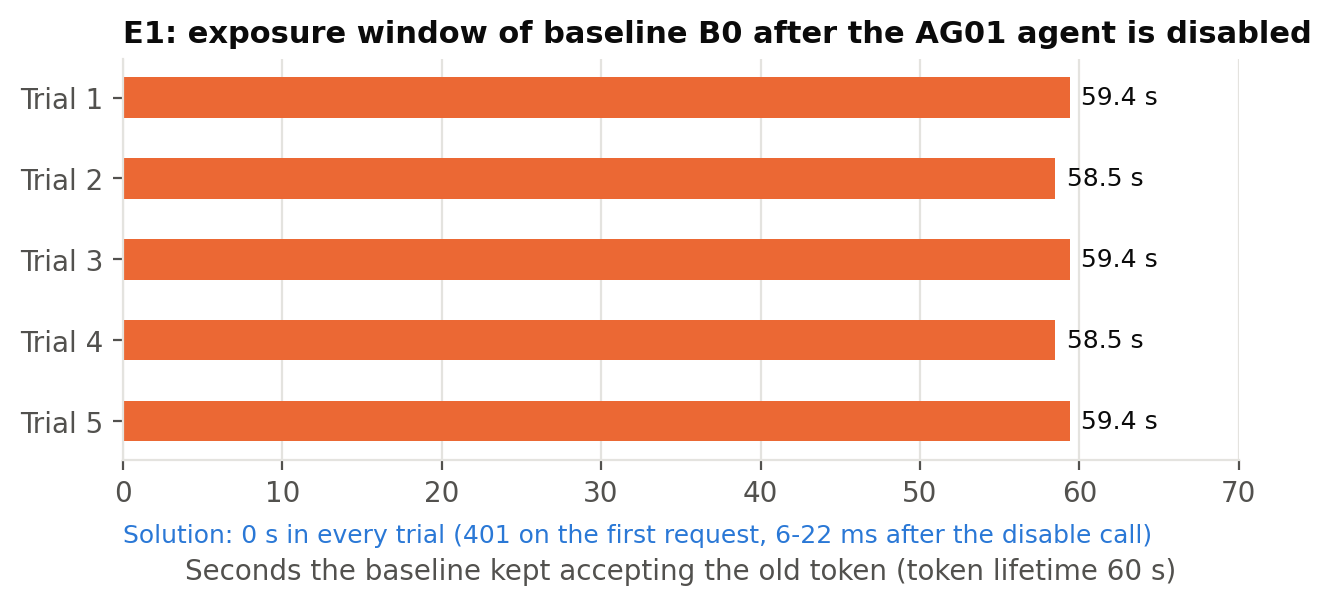
\includegraphics[width=0.49\textwidth]{e1-agent-exposure-window.png}
\caption{Left: trials in which the revoked token was accepted on the first request. Right: B0 keeps accepting a disabled agent's token for almost its whole 60\,s life; ours refuses it immediately.}
\end{figure}
\textbf{Observations.} B0 cannot see revocation at all. For 300\,s human web tokens its exposure would be up to five minutes. Our API met the frozen threshold in all 15 revocation trials. \textbf{Failure we disclose:} the control shows that \emph{neither} validator ends a session on password reset alone. That is Keycloak behaviour, measured and already in the frozen protocol, and it is why incident response must call logout-all.

\subsection*{Q1, Q2, Q5, Q6: the final clean-clone run of \texttt{e13f019} (14 Nov 2026)}
\begin{table}[H]
\centering\small
\begin{tabularx}{\textwidth}{@{}P{5.0cm} L@{}}
\toprule
\textbf{Check (expected)} & \textbf{Observed} (raw: \gh{docs/evidence/2026-11-14}{\code{docs/evidence/2026-11-14/}})\\
\midrule
Stack starts from a clean clone & 5/5 services healthy in 68\,s, 5 migrations and seed from scratch\\
Typecheck, build, \code{npm audit}, client config & pass, pass, 0 vulnerabilities, 9/9\\
Full suite, real PostgreSQL + live Keycloak (0 fail, 0 skip) & \textbf{253 passed, 0 failed, 0 skipped}, 11 files, 18.8\,s\\
Mutation runner (all killed; DB down $\Rightarrow$ exit 2) & \textbf{15/15 killed}, 0 survived; database stopped $\Rightarrow$ \textsc{inconclusive}, exit 2\\
Real-browser proof (11/11, 2 hosts) & \textbf{11/11} on \code{localhost} and \textbf{11/11} on \code{127.0.0.1} with no source change\\
AG02 outcomes (Q6) & 26 tests (4 live): no delegation 403; in scope 200; scope without user permission 403; user permission without scope 403; other tenant 403; admin scopes not delegable (400); revoked 401 on the first request (17\,ms)\\
Edge cases & cross-tenant ID $\Rightarrow$ 404; suspended member $\Rightarrow$ 403 but may withdraw consent; provider outage $\Rightarrow$ 503 (not 401); unsafe config $\Rightarrow$ process refuses to start; refresh replay kills the family; 12 concurrent first logins $\Rightarrow$ 1 user\\
\bottomrule
\end{tabularx}
\caption{Expected vs observed results of the final run.}
\end{table}
\begin{figure}[H]
\centering
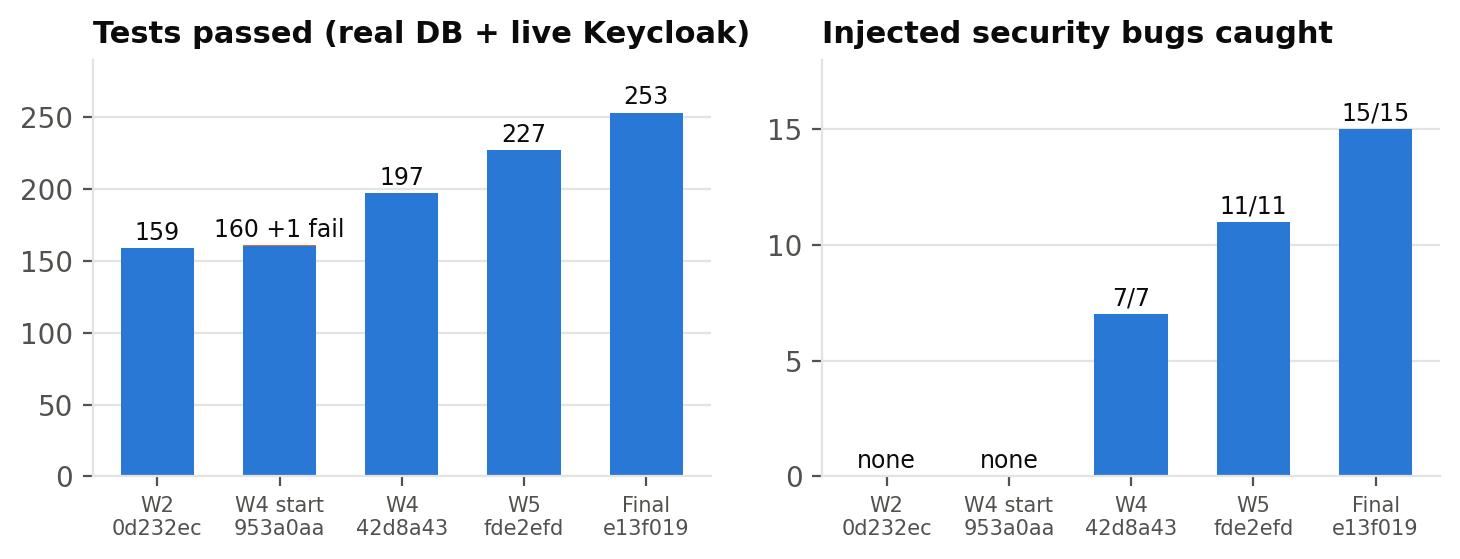
\includegraphics[width=0.53\textwidth]{verification-over-revisions.png}\hfill
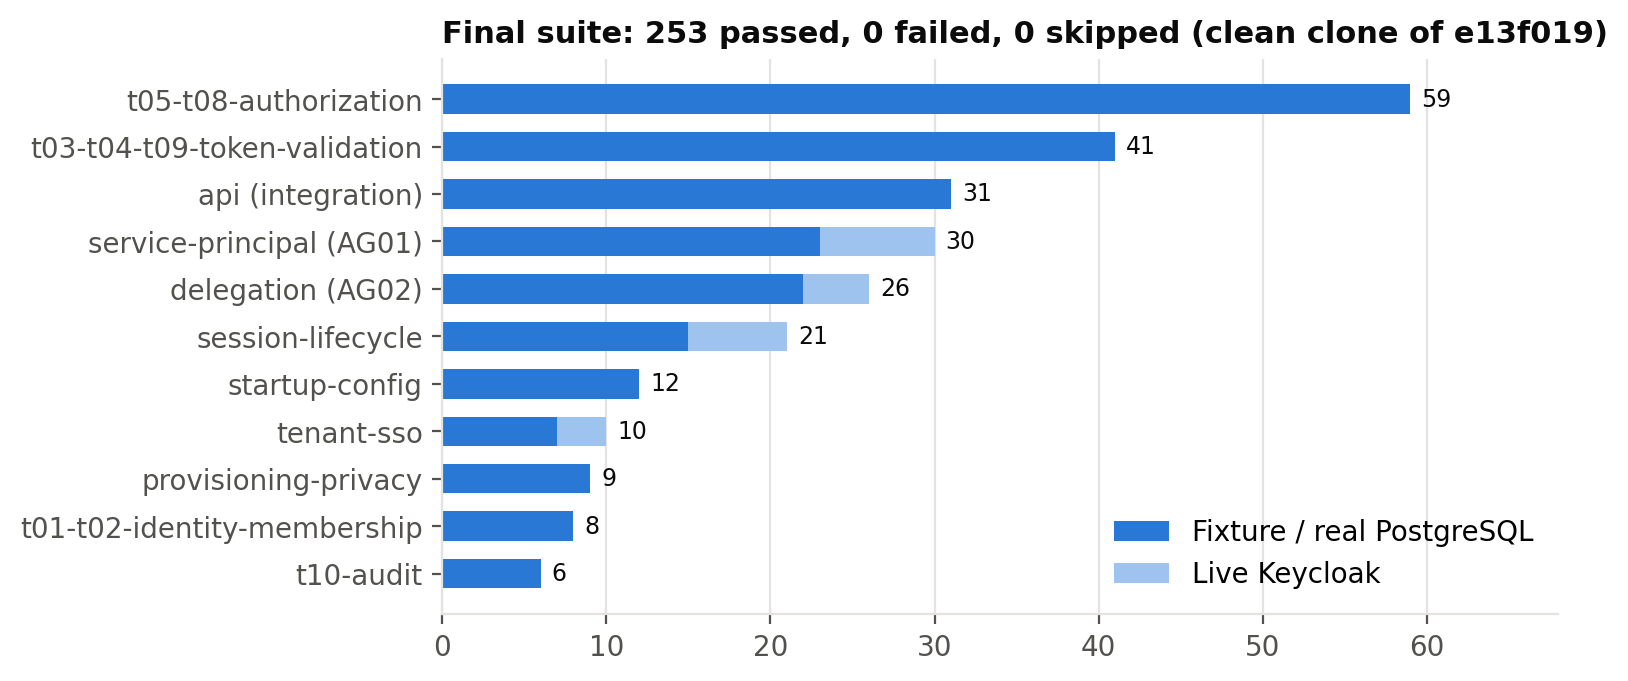
\includegraphics[width=0.45\textwidth]{final-suite-by-file.png}
\caption{Left: verification at each verified revision. The revision baseline \texttt{953a0aa} hid a real regression (1 failing test) that our earlier report had missed. Right: final suite by file (light = live provider).}
\end{figure}

\subsection*{Q4: cost of the check}
\begin{minipage}[t]{0.47\textwidth}\vspace{0pt}\small
\begin{tabular}{@{}lcc@{}}
\toprule
\textbf{Series} & \textbf{p50 (ms)} & \textbf{p95 (ms)}\\
\midrule
B0 local JWT verify & 0.15 & 0.28\\
\code{GET /health} (no auth) & 0.65 & 1.54\\
Introspection alone & 3.29 & 5.58\\
Full agent request (ours) & 9.25 & 15.14\\
\bottomrule
\end{tabular}\\[4pt]
Introspection is about a third of an authenticated request. That is the measured price of the Q3 result. These are sequential, single-machine observations, not a benchmark; nothing was optimised.
\end{minipage}\hfill
\begin{minipage}[t]{0.5\textwidth}\vspace{0pt}
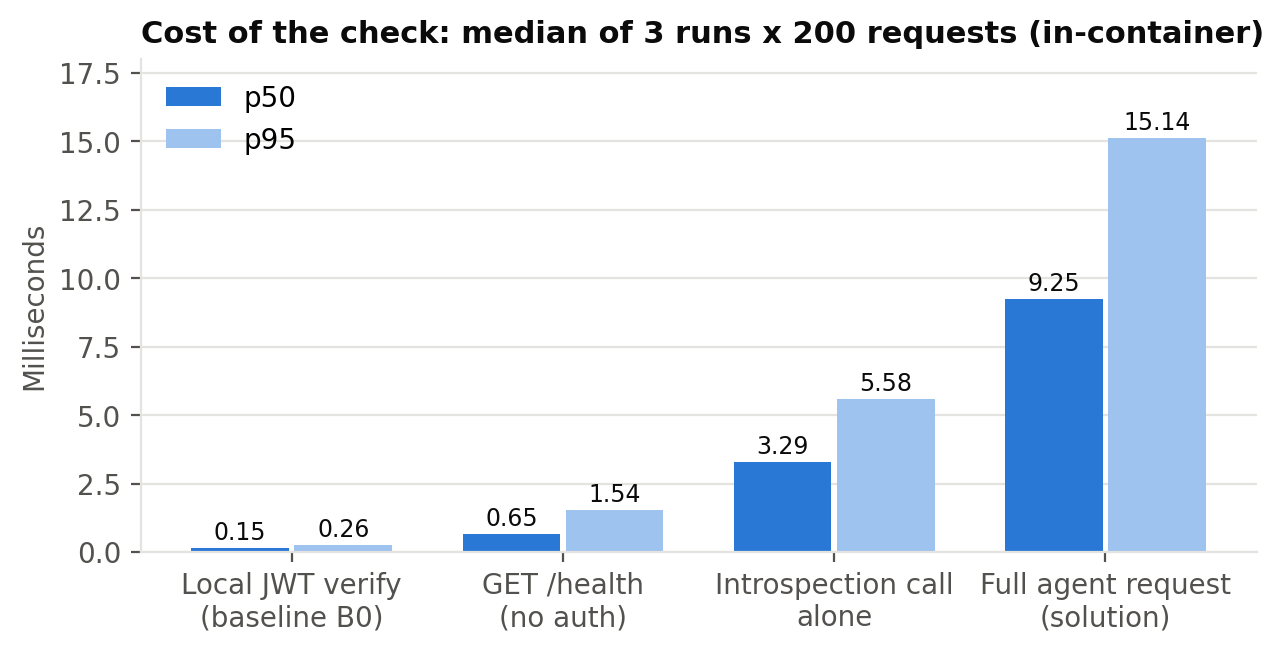
\includegraphics[width=\textwidth]{latency-cost.png}
\end{minipage}

\textbf{Conclusions supported by evidence.} (i) Every frozen acceptance criterion is met on a clean clone of the final revision. (ii) The tests can fail: each of 15 security guards, when removed, is caught by named tests. (iii) Compared with B0, uncached introspection turns ``valid until expiry'' (up to 60\,s for agents, 300\,s for users) into refusal on the next request, at about 3\,ms per request. \textbf{Tests not run:} an independent second-machine rerun; concurrency or throughput load; iOS/Safari; the physical-phone run (7 Nov, Android) predates AG02. E1 ran on the development stack and was repeated in a clean clone of the submission commit (16 Nov) with the same verdicts (\gh{evaluation/results/2026-11-16-clean}{raw logs}); that clean run's browser-proof and mutation steps did not complete (host low on memory), so their evidence is the 14 Nov run of identical code.

%% ---------------------------------------------------------------- 8
\section*{8. Current state, limitations \& risks}
\begin{table}[H]
\centering\small
\begin{tabularx}{\textwidth}{@{}P{2.0cm} L@{}}
\toprule
\textbf{Working} & M1--M4, M6, M7, AG01, AG02 as specified; web + mobile-style clients; enterprise broker; session listing and revocation; provisioning with tenant SSO association; mutation runner; evaluation scripts\\
\textbf{Partial} & M5 is a minimal slice (no SCIM \code{/Users}, \code{/Groups}; domains not DNS-verified); policy API can add allow/deny rows but not delete; AG01 grants only via seed/DB (no grant API); no admin view of others' delegations; delegation uses a custom header rather than an RFC~8693 token\\
\textbf{Missing} & native Android/iOS apps; real corporate IdP or SAML; production deployment (TLS, managed secrets, rate limiting, backups); independent second-machine reproduction; CI\\
\bottomrule
\end{tabularx}
\caption{Implementation status (actual, not intended).}
\end{table}
\textbf{Known failure modes and risks.} \emph{Availability:} if Keycloak is down every authenticated request gets 503 (fail closed by design). \emph{Consistency:} an already-authorized in-flight request may complete after a revocation; checks apply from the next request. \emph{Audit:} an ordinary table, not tamper-evident; provider revocations are logged as separate request/complete events. \emph{Security/privacy:} plain HTTP and public synthetic secrets (lab only); a phone over HTTP needs a Chrome secure-origin flag because PKCE uses \code{crypto.subtle}; no real user data is stored. \emph{Dependencies:} pinned images and lockfile; \code{npm audit} 0 on 14 Nov, but Keycloak advisories must be watched; re-enabling a disabled Keycloak client revives unexpired agent tokens, so the registry status is the reliable off switch. \emph{Process debts:} the evaluation protocol was frozen on 10 Oct, one day after the 9 Oct deadline (ADR-011); the Week~3 report over-claimed evidence that was later rebuilt (ADR-012). Open items are tracked as GitHub issues (\gh{docs/open-issues.md}{\code{docs/open-issues.md}}).

%% ---------------------------------------------------------------- 9
\section*{9. Way forward}
\begin{table}[H]
\centering\small
\begin{tabularx}{\textwidth}{@{}P{0.3cm} P{3.9cm} L P{4.1cm}@{}}
\toprule
\textbf{\#} & \textbf{Task (start here)} & \textbf{Rationale / dependencies} & \textbf{Done when}\\
\midrule
1 & Independent reproduction + CI\newline(\code{evaluation/} scripts) & Every number comes from one machine; needs a Docker-capable runner & a second machine and a CI job produce 253/0/0, 15/15 and E1 with the same verdicts\\
2 & Agent and policy administration API\newline(\code{service-principal}, \code{delegation} modules, \code{routes.ts}) & Grants are DB-only; admins cannot see delegations or delete rules & audited endpoints with tests; mutation for each new guard killed\\
3 & RFC 8693 delegation tokens\newline(\code{delegation} module) & Interoperability with external agents; Keycloak 26 supports standard token exchange & an exchanged token with an \code{act} claim works and revocation of the record still gives 401 on the next request\\
4 & SCIM 2.0 \code{/Users}, \code{/Groups} + DNS domain verification\newline(\code{provisioning} module) & Enterprises need automatic joiners/leavers & SCIM compliance tests pass; a deprovisioned user's next request is 403\\
5 & Production hardening\newline(\code{docker-compose.yml}, realm JSON) & TLS, secrets, rate limits, immutable audit sink & deployed over HTTPS with rotated secrets; browser proof 11/11 against it; no HTTP flag on phones\\
\bottomrule
\end{tabularx}
\caption{Prioritized next tasks. No technical blocker for \#1; it needs a second Docker-capable machine.}
\end{table}

%% ---------------------------------------------------------------- 10
\section*{10. Contributions, AI use \& attribution}
\textbf{Contributions.} \emph{Krishna Teja:} all 23 commits in the history (\href{\repo/commits/cs5903-final-2026}{commit list}), covering the backend modules and migrations (\commit{0d232ec}), the Week~2--4 fixes (\commit{f68add3}, \commit{5e4367a}, \commit{ece833d}, \commit{42d8a43}), AG01 (\commit{fde2efd}), AG02 (\commit{e13f019}), the realm configuration, clients, tests, mutation runner, evidence runs, reports and this evaluation, plus the physical phone run. \emph{Jaya Prakash:} no commits are authored by Jaya Prakash. The Week~4 plan assigned the phone run and an independent second-machine rerun to Jaya Prakash; the phone run was done by Krishna Teja and the rerun was not done. \JayaContribution{} Both members are responsible for explaining a request path, source code, a test and a trade-off in the viva.

\textbf{AI use and how it was checked.} An AI coding agent (Claude, Anthropic) was used throughout for code, tests, documentation and this submission package, including the E1 experiment script, figures and recorded demo. Its errors were plausible rather than random: a checker that could not fail, a test against an ID that could never match, answers describing intended rather than actual behaviour. The final report records 36 such issues. Every claim here was checked by running it on real infrastructure from a clean state, by mutation testing and by reading raw logs rather than summaries.

\textbf{Third-party assets.} Only the open-source components listed in \S2, used under their licences through package managers and official images; no copied code, no unlicensed assets; all data synthetic. The repository has no licence file yet; it is an academic submission.

%% ---------------------------------------------------------------- refs
\begin{thebibliography}{9}\small
\setlength{\itemsep}{0pt}
\bibitem{oidc} N.~Sakimura et al. \emph{OpenID Connect Core 1.0}. OpenID Foundation, 2014.
\bibitem{bcp} T.~Lodderstedt et al. \emph{RFC 9700: Best Current Practice for OAuth 2.0 Security}. IETF, 2025.
\bibitem{zanzibar} R.~Pang et al. Zanzibar: Google's consistent, global authorization system. \emph{USENIX ATC}, 2019.
\bibitem{scim} P.~Hunt et al. \emph{RFC 7644: System for Cross-domain Identity Management: Protocol}. IETF, 2015.
\bibitem{nist} NIST. \emph{Privacy Framework, Version 1.0}. 2020.
\bibitem{rfc8693} M.~Jones et al. \emph{RFC 8693: OAuth 2.0 Token Exchange}. IETF, 2020.
\bibitem{tools} Keycloak 26.8.0 (keycloak.org); Casbin (casbin.org); Fastify (fastify.dev); Playwright (playwright.dev).
\end{thebibliography}

\subsection*{Appendix: where to find everything}
\small
\begin{tabularx}{\textwidth}{@{}P{4.4cm} L@{}}
\toprule
Setup, run, test, handover & \gh{README.md}{\code{README.md}}\\
ADR log (incl.\ 9 Oct methodology record) & \gh{docs/Architecture_Decision_Records.md}{\code{docs/Architecture\_Decision\_Records.md}}\\
Evaluation scripts, raw results, figures & \gh{evaluation/README.md}{\code{evaluation/}}\\
Evidence by revision and date & \gh{docs/verification-evidence.md}{\code{docs/verification-evidence.md}}, \gh{docs/evidence}{\code{docs/evidence/}}\\
Requirements traceability; mentor feedback & \gh{docs/traceability-matrix.md}{\code{docs/traceability-matrix.md}}, \gh{docs/mentor-responses.md}{\code{docs/mentor-responses.md}}\\
Long final report (61 pages, 36 issues and fixes) & \gh{docs/Final_Report_Full.pdf}{\code{docs/Final\_Report\_Full.pdf}} (source \gh{final_report.tex}{\code{final\_report.tex}})\\
Demo recording; presentation & \gh{docs/demo/demo-walkthrough.mp4}{\code{docs/demo/demo-walkthrough.mp4}}; \gh{docs/Final_Presentation.pptx}{\code{docs/Final\_Presentation.pptx}}\\
\bottomrule
\end{tabularx}
\end{document}
